\chapter{Instalación del clúster \label{sec:implementacion}}

\section{Introducción}
En este apartado se detallarán los aspectos relevantes para la implementación de la arquitectura \textit{big data} diseñada en el apartado \ref{sec:disenho}.

Como se indica en dicho apartado, se plantean una configuracion para el sistema multinodo, donde una máquina es el maestro y, el resto, los esclavos.

Por tanto, se comentaran todos los detalles y pasos para montar la arquitectura diseñada y, de esta forma, conseguir un sistema \textit{big data} funcional y completo que sea capaz de almacenar, procesar y analizar los datos para obtener las respuestas de las consultas planteadas.

\section{Preparación del entorno de trabajo}
Como se expuso en el apartado \ref{sparkEA}, donde se habla de \textit{Apache Spark}, este, resulta compatible con las tres sistemas operativos más importantes para ordenadores, aunque la solución escogida ha sido Linux para ejecutarlo. Se va a utilizar Ubuntu Desktop \cite{ubuntu} para el master y Ubuntu Server para los slaves. 

Aunque se podría ejecutar todo el clúster exclusivamente en un entorno Ubuntu Server, se ha decidido utilizar la variante Desktop en el master para poder realizar los análisis directamente desde el nodo.

\subsection{Especificaciones del equipo \label{eqEspec}}
\begin{table}[htp!]
	\centering
	\caption{Especificaciones del maestro}
	\label{maestro}
	\begin{tabular}{|l|l|}
		\hline
		\multicolumn{2}{|c|}{\textbf{GENERAL}}                                 \\ \hline
		\textbf{Nombre:}            & david-hdp		                           \\ \hline
		\textbf{Sistema Operativo:} & Linux                                    \\ \hline
		\textbf{Versión:}           & Ubuntu 16.10 (64 bits)                   \\ \hline
		\textbf{Usuario:}           & david                         	       \\ \hline
		\multicolumn{2}{|c|}{\textbf{SISTEMA}}                                 \\ \hline
		\textbf{Procesador:}        & Intel(R) Core(TM) i7-3820 CPU @ 4.30GHz  \\ \hline
		\textbf{Cores:}             & 8                                        \\ \hline
		\textbf{Threads por core:}  & 2                                        \\ \hline
		\textbf{RAM:}               & 16384                                    \\ \hline
		\multicolumn{2}{|c|}{\textbf{ALMACENAMIENTO}}                          \\ \hline
		\textbf{Dispositivo:}       & Kingston SUV400S37480G                   \\ \hline
		\textbf{Tamaño:}            & 1 Tb	                                   \\ \hline
		\multicolumn{2}{|c|}{\textbf{RED}}                                     \\ \hline
		\textbf{Dispositivo:}       & Realtek PCIe GBE Family Controller       \\ \hline
		\textbf{Nombre:}            & Master                                   \\ \hline
	\end{tabular}
\end{table}

\begin{table}[htp!]
	\centering
	\caption{Especificaciones del nodo1}
	\label{esclavo}
	\begin{tabular}{|l|l|}
		\hline
		\multicolumn{2}{|c|}{\textbf{GENERAL}}                             			    \\ \hline
		\textbf{Nombre:}            & node1			                         			\\ \hline
		\textbf{Sistema Operativo:} & Linux                                   			\\ \hline
		\textbf{Versión:}           & Ubuntu 16.10 (64 bits)                   			\\ \hline
		\textbf{Usuario:}           & david                         	       			\\ \hline
		\multicolumn{2}{|c|}{\textbf{SISTEMA}}                                 			\\ \hline
		\textbf{Procesador:}        & Intel(R) Celeron(TM) T1600 @ 2GHz  	\\ \hline
		\textbf{Cores:}             & 2                                        			\\ \hline
		\textbf{Threads por core:}  & 1                                        			\\ \hline
		\textbf{RAM:}               & 	8192                                    			\\ \hline
		\multicolumn{2}{|c|}{\textbf{ALMACENAMIENTO}}                          			\\ \hline
		\textbf{Dispositivo:}       & Samsung HM320JI\\ \hline
		\textbf{Tamaño:}            & 320 Gb	                                   			\\ \hline
		\multicolumn{2}{|c|}{\textbf{RED}}                                     			\\ \hline
		\textbf{Dispositivo:}       & Realtek PCIe GBE Family Controller       			\\ \hline
		\textbf{Nombre:}            & node1                                  			\\ \hline
	\end{tabular}
\end{table}

\clearpage
\subsection{Instalación del sistema operativo}
Esta instalación solo fue necesaria de llevar a cabo en los esclavos que utilizaríamos para el entorno doméstico. Como se ha comentado anteriormente, el \gls{SO} elegido será Ubuntu, concretamente, la versión 16.10.

\subsubsection{Requisitos previos}
Para proceder con la instalación del sistema operativo en los ordenadores había que cumplir algunos requisitos muy básicos. Lo primero era contar con máquinas que superasen los requisitos mínimos \cite{ubuntu} necesarios para su correcta ejecución, cosa que las utilizadas cumplían (especificaciones en el apartado \ref{eqEspec}). 


También sería necesario un soporte de instalación del \gls{SO}, que en este caso fue un \gls{DVD}), en el que se grabó una imagen con Ubuntu, que permitió el inicio de este sistema operativo en las máquinas y su posterior instalación en ellas, de forma local en el disco duro.

\subsection{Instalación de Apache Spark}
Para la realización de este proyecto utilizaremos la versión 2.2.0 \textit{Apache Spark}, que era la versión disponible cuando se comenzó a trabajar en él. Como lo que se deseaba era una versión estable para realizar todo el trabajo, se descartó la creación del paquete a partir del código fuente y, también, la actualización a la versión 2.2.1 que salió en diciembre. 

Por tanto, para la instalación de \textit{Apache Spark} en los equipos que se utilizarían se recurrió a la versión pre-compilada del \Gls{framework} \cite{descargaSpark}, en concreto la compilada para funcionar con \textit{Apache Hadoop 2.9} que se utilizaría en la configuración multinodo del clúster.


\subsubsection{Prerrequisitos}
Para que \textit{Apache Spark} funcione de forma correcta en el sistema se necesita cumplir una serie de prerrequisitos:

\begin{itemize}
	\item Tener instalado Linux en el sistema.
	\item Tener instalado Java en el sistema.
	\item Tener instalado Scala \cite{scala} en el sistema.
	\item Tener instalado Python en el sistema.
	\item Tener instalado SSH en el sistema.
	\item Disponer de un usuario y grupo común en todas las máquinas.
\end{itemize}


\subsubsection{Instalación de Java y Scala}
La instalación de estos dos lenguajes es esencial para el funcionamiento de \textit{Apache Spark} debido a que está escrito en Scala. Por otro lado, Java es necesario ya que Scala \cite{scala} necesita de la \gls{JVM} para su funcionamiento.

La instalación de estos dos lenguajes de programación se realiza a través de la terminal de forma muy sencilla, primero se añade el repositorio oficial de Oracle \cite{descargaJava} y posteriormente se introduce los comandos de instalación.
Los comandos necesarios se encuentran en el bloque de código \ref{ins:java}.

\begin{lstlisting}[label=ins:java,language=sh,frame=single, caption=Instalación de Java y Scala.]
sudo add-apt-repository ppa:webupd8team/java
sudo apt-get update
sudo apt-get install oracle-java8-installer
sudo apt install scala
\end{lstlisting}

\subsubsection{Instalación de Anaconda (Python)}
Python va a ser esencial para el desarrollo de este proyecto ya que se utilizará la \gls{API} en este lenguaje para escribir todo el código que procese \textit{Apache Spark}, conocida como \textit{PySpark}. Además como \gls{IDLE} utilizaremos \textit{Jupyter Notebook} \cite{jupyter}, que es ampliamente conocido en el entorno de la ciencia de datos.

Para instalar tanto Python como \textit{Jupyter Notebook} vamos a utilizar una distribución, que contiene estos y además muchas otras librerías útiles, llamada \textit{Anaconda} \cite{anaconda}. La instalación se realizara en la carpeta \textit{``/opt''} del sistema.
Los comandos necesarios para la instalación se encuentran en el bloque de código \ref{ins:anaconda}.

\begin{lstlisting}[label=ins:anaconda,language=sh,frame=single, caption=Descarga e instalación de Anaconda.]
sudo wget https://repo.continuum.io/archive/Anaconda3-5.0.1-Linux-x86_64.sh
sudo bash Anaconda3-5.0.1-Linux-x86_64.sh
\end{lstlisting}

\subsubsection{Creación de usuario y grupo común \label{grupoComun}}
Para evitar posibles problemas de permisos durante la ejecución de las tareas, es buena práctica tener un grupo de usuarios donde estén las máquinas incluidas en el clúster.

Por tanto, para abordar este problema, durante la instalación del \gls{SO} en las máquinas del clúster se estableció el mismo nombre de usuario para todas. Además, tras esta se creo un nuevo grupo de usuarios, donde se incluyó a dichos usuarios. El proceso para la creación del grupo y adición del usuario a este se puede encontrar en el fragmento de código \ref{usuarioGru}

\clearpage
\begin{lstlisting}[label=usuarioGru,language=sh,frame=single,caption=Creación de grupo común y adición del usuario del sistema a este.]
sudo addgroup spark
sudo adduser --ingroup spark david
\end{lstlisting}

Una vez realizados estos pasos, las máquinas de la red tendrían acceso a los ficheros de cualquier otra si el grupo tuviese permisos de acceso en dichos archivos. En este caso, todo el conjunto de ficheros utilizados por el sistema \textit{big data} tendrá acceso de lectura y escritura por el grupo de usuarios \textit{spark}, como se explicará en la configuración de \textit{Apache Spark}.

\subsubsection{Instalación de \gls{SSH} y creación del certificado \label{insSSH}}
El cliente de \gls{SSH} viene instalado por defecto en Ubuntu y Debian, sin embargo, para que los nodos devuelvan la llamada del maestro y establecer la conexión cuando se inicie el clúster, será necesario que estos dispongan del servidor \gls{SSH}. 

Estos programas también se encuentran en el repositorio oficial de Ubuntu, por lo que la instalación se realiza escribiendo el nombre del paquete en la terminal. Con respecto a los equipos de la universidad, estos están ya instalados para su uso. El comando de consola para instalarlo se encuentra en el fragmento de código \ref{ins:ssh}.

\begin{lstlisting}[label=ins:ssh,language=sh,frame=single,caption=Instalación del cliente y el servidor de \gls{SSH}.]
sudo apt install openssh-client
sudo apt install openssh-server
\end{lstlisting}

Una vez instalados los programas, el siguiente paso será crear el certificado \gls{SSH} para cada equipo y, así, facilitar las conexiones entre los nodos. Es decir, una vez creado los certificados \gls{SSH} de cada máquina, si estos son compartidos entre ellas, los equipos pasarán a estar en la lista de dispositivos seguros y no será necesaria la autentificación con contraseña para establecer la conexión.

El proceso de creación de certificados se puede encontrar en el fragmento de código \ref{confCert} y se realizará en todos las máquinas.

\begin{lstlisting}[label=confCert,language=sh,frame=single,caption=Creación y autorización del certificado \gls{SSH}.]
ssh-keygen -t rsa -P ""
cat $HOME/.ssh/id_rsa.pub >> $HOME/.ssh/authorized_keys
\end{lstlisting}

Tras estos pasos, ya tenemos los prerrequisitos completos para iniciar la instalación del clúster.

\clearpage
\subsubsection{Instalación y configuración del modo distribuido}
Este apartado se tratará la configuración de \textit{Apache Spark} para la configuración distribuida o multinodo, donde existe una máquina que hará de maestro y $n$ máquinas que harán de esclavos. 

\paragraph{Asignación de IPs y nombres de sistema en la red.}
Este proceso se realizará para simplificar la conexión entre los nodos de los sistemas utilizados, permitiendo con ellos, realizar las conexiones \gls{SSH} mediante el uso de los nombres asignados, en vez de las direcciones  
IP locales.

En este caso se realizará modificando el archivo ``/etc/hosts'' en cada nodo utilizado. Como se tenemos dos equipos el \textit{master} recibirá el nombre de ``david-hdp'' que es el nombre que tenía anteriormente y el esclavo será \textit{nodo n} donde $n$ será su número de esclavo en el sistema. La modificación del archivo ``hosts'' será la misma para todos los nodos, añadiendo las líneas que se encuentran en el fragmento de código \ref{confhosts}

\begin{lstlisting}[label=confhosts,language=sh,frame=single,caption=Líneas a añadir en el fichero ``/etc/hosts'' de cada nodo del clúster.]
192.168.1.15 	david-hdp
192.168.1.17	node1
\end{lstlisting}

\paragraph{Compartición de certificados \gls{SSH}.}
Como se indicó en el apartado \ref{insSSH}, la creación de los certificados \gls{SSH} permitirá que, al compartirse entre los equipos que formen el clúster, no sea necesaria la autentificación con contraseña, simplificando el proceso de conexión entre las máquinas. Además este proceso es requerido tanto por \textit{Apache Spark} como por \textit{Apache Hadoop} para realizar la interoperatividad.

En el caso del entorno doméstico, será el maestro el que necesite los certificados de los esclavos para realizar la conexión, por lo que el proceso seguido es la copia de estos en el nodo maestro. El proceso inverso y la compartición entre esclavos no será necesaria, ya que, es el maestro el que inicia la conexión y porque los esclavos no están conectados entre sí.

Es exclusivamente el maestro el que requiere certificarse en los esclavos para realizar la conexión, por lo que el proceso seguido es la copia de estos en el nodo maestro. El proceso inverso y la adición entre esclavos no será necesaria, ya que, es el maestro el que inicia la conexión y los esclavos no están interconectados.

Los comandos a ejecutar en la terminal del nodo maestro para la obtención de los certificados de los esclavos se puede encontrar en el fragmento de código \ref{comandosSSH}.

\begin{lstlisting}[label=comandosSSH,language=sh,frame=single,caption=Obtención de los certificados \gls{SSH} de los esclavos por parte del maestro en el clúster.]
ssh-copy-id -i $HOME/.ssh/id_rsa.pub david@node1
\end{lstlisting}

Por último, para evitar que el servidor \gls{SSH} rechace las peticiones de forma automática editaremos el fichero ``/etc/ssh/sshd\_config'', la modificación será reflejada en el fragmento de código \ref{confsshd}.

\begin{lstlisting}[label=confsshd,language=sh,frame=single,caption=Líneas modificadas en el fichero ``/etc/ssh/sshd\_config'' cada nodo del clúster.]
PasswordAuthentication No
\end{lstlisting}

Posteriormente para hacer efectivo el cambio se ejecutará el comando que se puede encontrar en el fragmento de código \ref{sshdrestart} o simplemente reiniciando el equipo.

\begin{lstlisting}[label=sshdrestart,language=sh,frame=single,caption=Comando de consola para reiniciar el servidor \gls{SSH}.]
sudo service sshd restart
\end{lstlisting}

\paragraph{Instalación de \textit{Apache Spark}.}
La instalación de \textit{Apache Spark} en este caso se tiene que hacer de forma manual en cada máquina del sistema,
Para la realización de este proceso de forma automática en cada nodo se creó un script que se ejecutaría en cada nodo del sistema \textit{big data}. El código de este se puede encontrar en el fragmento de código \ref{insSpark}.

\begin{lstlisting}[label=insSpark,language=sh,frame=single,caption=Script de instalación de \textit{Apache Spark}.]
#!/bin/bash
cd /opt
wget http://apache.uvigo.es/spark/spark-2.2.0/spark-2.2.0-bin-hadoop2.7.tgz
tar -xvzf spark-2.2.0-bin-hadoop2.7.tgz 
mv spark-2.2.0-bin-hadoop2.7 spark
rm -rf spark-2.2.0-bin-hadoop2.7.tgz
chmod 1777 -R /opt/spark
\end{lstlisting}

\paragraph{Configuración de \textit{Apache Spark}.}
El primer paso a realizar es indicar al sistema la ruta de instalación de \textit{Apache Spark} y de Java, modificando el archivo ``.bashrc'' de cada nodo. Debido a que el nombre de usuario es el mismo en todos los equipos, el fragmento de código a añadir en el fichero es el mismo para todos, siendo este el que se puede encontrar en el código \ref{confBash}. Se puede ver el fichero ``.bashrc'' completo en el anexo \ref{sc:bashrc}.

Por otro lado, también hay que modificar los archivos de configuración de \textit{Apache Spark} para su correcto funcionamiento los cuales se pueden encontrar en ``/opt/spark/conf''. Primero se modificará el archivo ``spark-env.sh'' en todos los nodos, para establecer que máquina será la maestra y donde se ha instalado java y python. Estas últimas líneas no serían necesarias, dado que debería haberse añadido esta variable de sistema durante la instalación de java.
\clearpage
\begin{lstlisting}[label=confBash,language=sh,frame=single,caption=Líneas a añadir en el fichero ``spark-env.sh'' para configurar \textit{Apache Spark} en el modo distribuido.]
export SPARK_MASTER_IP=david-hdp # Nombre del maestro del cluster
export JAVA_HOME=/usr/lib/jvm/java-8-oracle
export HADOOP_CONF_DIR=/opt/hadoop/etc/hadoop

export SPARK_WORKER_INSTANCES=1
export SPARK_DRIVER_MEMORY=2G
export PYSPARK_PYTHON=/opt/anaconda3/bin/python3.6
export PYSPARK_DRIVER_PYTHON=/opt/anaconda3/bin/python3.6
\end{lstlisting}

Por último, a partir de la versión 2.0 de \textit{Apache Spark} las configuraciones genéricas ya no se realizan en el fichero ``spark-env.sh'' sino en el fichero ``spark-defaults.conf'', en nuestro caso el contenido de dicho fichero es el especificado en el fragmento de código \ref{sparkDefaults}.

\begin{lstlisting}[label=sparkDefaults,language=sh,frame=single,caption=Contenido del fichero ``spark-defaults.conf'' de configuración de \textit{Apache Spark}.]
spark.master                     spark://david-hdp:7077
spark.eventLog.dir               hdfs:///spark-history
spark.eventLog.enabled           true
spark.history.fs.logDirectory    hdfs:///spark-history
spark.history.provider           org.apache.spark.deploy.history.FsHistoryProvider
spark.history.ui.port            18080
spark.executor.memory            2G
spark.executor.cores             2
\end{lstlisting}

Tras realizar esto, el siguiente paso, será establecer que máquinas de la red formarán parte del clúster. Esto se indicará en el archivo  ``/opt/spark/conf/slaves'', donde se escribirá el nombre de red de los nodos que se utilizarán. En este caso, al ser el maestro también un esclavo se le incluirá en dicho fichero, en un clúster de producción el maestro no sería en ningún caso esclavo, es más, existirían dos maestros para prevenir la caída de uno de ellos. Las líneas a añadir en el fichero se puede encontrar en el fragmento de código \ref{slaves} que solo será necesario escribir en el nodo maestro, que será el que realice las conexiones.

\begin{lstlisting}[label=slaves,language=sh,frame=single,caption=Líneas a añadir en el fichero ``slaves'' para establecer las máquinas a utilizar en el clúster.]
localhost # Es la maquina maestra
node1
\end{lstlisting}

\clearpage
\subsection{Configuración de \textit{Jupyter Notebook}}
Como se ha comentado anteriormente en la sección \ref{jupyterEA} se va a utilizar como \gls{IDLE} \textit{Jupyter Notebook}. Para poder utilizar PySpark en \textit{Jupyter} se ha de crear un nuevo kernel, para ello ser hará uso del código \ref{jupyterfile} y se escribirán las líneas reflejadas en el fragmento \ref{jupyterKernel}. 

\begin{lstlisting}[label=jupyterfile,language=sh,frame=single,caption=Comando para generar el kernel \textit{Jupyter} para PySpark.]
sudo mkdir -p /opt/anaconda3/share/jupyter/kernels/pyspark
sudo nano /opt/anaconda3/share/jupyter/kernels/pyspark/kernel.json
\end{lstlisting}

\begin{lstlisting}[label=jupyterKernel,frame=single,caption=Contenido del fichero ``kernel.json'' para la configuración con \textit{Apache Spark}.]
{
	"display_name": "PySpark",
	"language": "python",
	"argv": [
		"/opt/anaconda3/bin/python3",
		"-m",
		"ipykernel",
		"-f",
		"{connection_file}"
	],
	"env": {
		"SPARK_HOME": "/opt/spark/",
		"PYTHONPATH": "/opt/spark/python:/opt/spark/python/lib/py4j-0.10.4-src.zip",
		"PYTHONSTARTUP": "/opt/spark/python/pyspark/shell.py"
	}
}
\end{lstlisting}

La variable asociada al ``pythonpath'' del fragmento \ref{jupyterKernel} puede variar según la versión de \textit{Apache Spark} por lo que sería necesario comprobar si corresponde a la instalada. En este caso, debido a la versión que hemos utilizado la numeración del fichero es la correcta.

\clearpage
\subsection{Instalación de \textit{Apache Hadoop}\label{hadoopCluster}}

Como se ha indicado en el diseño de la arquitectura \textit{big data}, en el apartado \ref{sec:disenho}, para la configuración distribuida del clúster se necesita un mecanismo de replicación de datos para su funcionamiento. Por tanto, como se explicó, se decidió usar \textit{Apache Hadoop}, en concreto su sistema de ficheros distribuido, \gls{HDFS}, que permitirá la disponibilidad de las trazas en todos los nodos del clúster.

En este apartado se va a proceder a explicar el proceso de instalación y configuración de este sistema. La versión de \textit{Apache Hadoop} utilizada en este proyecto es la versión 2.9.0 precompilada, que está disponible para su descarga desde la página oficial \cite{descargaHadoop}.

Al tratarse de un sistema distribuido, al igual que con la instalación de \textit{Apache Spark}, esta deberá realizarse en cada sistema. Para agilizar este proceso, se ha creado un script para que realice la descarga del fichero ``.tar.gz'', lo descomprima y lo mueva a la ubicación seleccionada para su instalación. Esta ubicación será similar a la de \textit{Apache Spark}, es decir, será instalado en la ruta ``/opt/hadoop/''. El script ejecutado se encuentra en el fragmento de código \ref{insHadoop}.


\begin{lstlisting}[label=insHadoop,language=sh,frame=single,caption=Script de instalación de \textit{Apache Hadoop}.]
#!/bin/bash
wget http://www-us.apache.org/dist/hadoop/common/stable2/hadoop-2.9.0.tar.gz
tar -xzvf hadoop-2.9.0.tar.gz
mv hadoop-2.9.0/ /opt/hadoop
rm -rf hadoop-2.9.0.tar.gz
chmod 1777 -R /opt/hadoop
\end{lstlisting}

\paragraph{Estructura de carpetas para \textit{Apache Hadoop}.} Antes de iniciar la configuración de de \textit{Apache Hadoop} vamos a crear la estructura de directorios de trabajos de \gls{HDFS} que configuraremos posteriormente. Como se ha explicado anteriormente en la sección \ref{hadoopEA}, existen dos tipos de nodo, \textit{datanode} y \textit{namenode}, el primero contiene los datos de replicación y no existe limitación en cuanto a su número, mientras el segundo tipo es un nodo de control o nodo maestro. 

Esta diferencia es importante ya que se van a realizar dos estructuras diferentes según el tipo de nodo. Para el nodo maestro vamos a realizar la estructura que aparece reflejada en la figura \ref{fig:estructMaster}, los comandos para su realización se pueden ver en el fragmento de código \ref{cod:estructMaster}.

\begin{figure}[htp!] 
	\centering		
	\caption{Estructura de carpetas para operativa del \textit{namenode}.}
	\label{fig:estructMaster}
	\vspace{5pt}
	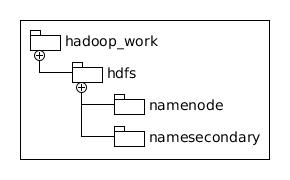
\includegraphics[scale=0.8]{graphics/estructMaster}
\end{figure}

\begin{lstlisting}[label=cod:estructMaster,language=sh,frame=single,caption=Codigo de creación de la estructura de carpetas del \textit{namenode}.]
sudo mkdir -p /opt/hadoop_work/hdfs/namenode
sudo mkdir -p /opt/hadoop_work/hdfs/namesecondary
\end{lstlisting}

Para los nodos esclavos se va a realizar la estructura de carpetas reflejada en la figura \ref{fig:estructSlave}. Para la realización de este proceso de forma automática en cada nodo se creó un script que se ejecutaría en cada nodo del sistema \textit{big data}. El código de este se puede encontrar en el fragmento de código \ref{cod:estructSlave}.

\begin{figure}[htp!] 
	\centering		
	\caption{Estructura de carpetas para operativa del \textit{datanode}.}
	\label{fig:estructSlave}
	\vspace{5pt}
	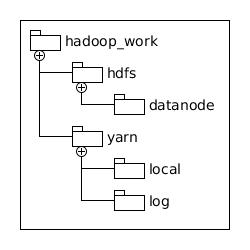
\includegraphics[scale=0.8]{graphics/estructSlave}
\end{figure}

\begin{lstlisting}[label=cod:estructSlave,language=sh,frame=single,caption=Codigo de creación de la estructura de carpetas del \textit{datanode}.]
#!/bin/bash
mkdir -p /opt/hadoop_work/hdfs/datanode
mkdir -p /opt/hadoop_work/yarn/local
mkdir -p /opt/hadoop_work/yarn/log
chown david:david -R /opt/hadoop_work/
\end{lstlisting}

\clearpage
\paragraph{Configuración de \textit{Apache Hadoop.}}
Tras la descarga e instalación de \textit{Apache Hadoop}, para su funcionamiento, será necesario modificar diferentes archivos de configuración. Lo primero será modificar los archivos de sistema para establecer correctamente las rutas de instalación y, posteriormente, los ficheros propios del \gls{framework}.

Como en el caso de la instalación de \textit{Apache Spark} el fichero de sistema a modificar es ``bashrc'', al que habrá que añadirle unas líneas indicando diferentes rutas de instalación de los módulos de \textit{Apache Hadoop} para su funcionamiento. Las lineas a añadir se pueden encontrar en el fragmento de código \ref{bashadoop}.

\begin{lstlisting}[label=bashadoop,language=sh,frame=single,caption=Líneas a añadir a ``.bashrc'' para el funcionamiento de \textit{Apache Hadoop}.]
export HADOOP_HOME=/opt/hadoop
export PATH=$PATH:$HADOOP_HOME/bin
export PATH=$PATH:$HADOOP_HOME/sbin
export HADOOP_CONF_DIR=$HADOOP_HOME/etc/hadoop
export HADOOP_MAPRED_HOME=$HADOOP_HOME
export HADOOP_COMMON_HOME=$HADOOP_HOME
export HADOOP_HDFS_HOME=$HADOOP_HOME
export HADOOP_YARN_HOME=$HADOOP_HOME
export YARN_HOME=$HADOOP_HOME
export HADOOP_COMMON_LIB_NATIVE=$HADOOP_HOME/lib/native
export HADOOP_OPTS="-Djava.library.path=$HADOOP_HOME/lib"
export CLASSPATH=$CLASSPATH:$HADOOP_HOME/lib/*
\end{lstlisting}

Posteriormente, se modificarán los diferentes ficheros de configuración de \textit{Apache Hadoop} para hacerlo funcionar en el clúster doméstico. Todos estos archivos residen en la ruta ``/opt/etc/hadoop''. Los ficheros a modificar serán los siguientes:

\begin{itemize}
\item \textbf{hadoop-env.sh:} Donde se indicará la ruta de instalación de Java en la máquina.
\begin{lstlisting}[label=hadoopenv,language=sh,frame=single,caption=Línea a añadir a ``hadoop-env.sh''.]
export JAVA\_HOME=/usr/lib/jvm/java-8-oracle
\end{lstlisting}

\item \textbf{core-site.xml}
\begin{lstlisting}[label=coresite,language=XML,frame=single,caption=Contenido del ``core-site.xml''.]
<configuration>
	<property>
		<name>fs.defaultFS</name>
		<value>hdfs://david-hdp:9000</value>
	</property>
	
	<property>
		<name>ipc.maximum.data.length</name>
		<value>134217728</value>
	</property>
	<property>
		<name>io.file.buffer.size</name>
		<value>131072</value>
	</property>
</configuration>
\end{lstlisting}

\item \textbf{hdfs-site.xml}
\begin{lstlisting}[label=hdfssite1,language=XML,frame=single,caption=Contenido del ``hdfs-site.xml'' de el nodo maestro.]
<configuration>
	<property>
		<name>dfs.replication</name>
		<value>2</value>
		<description>Replication factor, 1 no copy, 2 two copies each fragment</description> 
	</property>
	<property>
		<name>dfs.namenode.name.dir</name>
		<value>file:/opt/hadoop_work/hdfs/namenode</value>
		<description>Carpeta correspondiente al NameNode</description> 
	</property>
	<property>
		<name>dfs.datanode.data.dir</name>
		<value>file:/opt/hadoop_work/hdfs/datanode</value>
		<description>Carpeta correspondiente al DataNode</description> 
	</property>
	<property>
		<name>dfs.namenode.checkpoint.dir</name>
		<value>file:/opt/hadoop_work/hdfs/namesecondary</value>
		<description>Carpeta correspondiente al NameSecondary</description> 
	</property>
	<property>
		<name>dfs.block.size</name>
		<value>134217728</value>
		<description>Tamanno maximo de bloque de archivo (128Mb)</description> 
	</property>
	<property>
		<name>dfs.webhdfs.enabled</name>
		<value>true</value>
	</property>
</configuration>
\end{lstlisting}

\clearpage
\begin{lstlisting}[label=hdfssite2,language=XML,frame=single,caption=Contenido del ``hdfs-site.xml'' de los nodos esclavos.]
<configuration>
	<property>
		<name>dfs.replication</name>
		<value>2</value>
		<description>Replication factor, 1 no copy, 2 two copies each fragment</description> 
	</property>
	<property>
		<name>dfs.datanode.data.dir</name>
		<value>file:/opt/hadoop_work/hdfs/datanode</value>
		<description>Carpeta correspondiente al DataNode</description> 
	</property>
	<property>
		<name>dfs.namenode.checkpoint.dir</name>
		<value>file:/opt/hadoop_work/hdfs/namesecondary</value>
		<description>Carpeta correspondiente al NameSecondary</description> 
	</property>
	<property>
		<name>dfs.block.size</name>
		<value>134217728</value>
		<description>Tamanno maximo de bloque de archivo (128Mb)</description> 
	</property>
</configuration>
\end{lstlisting}

\item \textbf{ mapred-site.xml}
\begin{lstlisting}[label=mapredsite,language=XML,frame=single,caption=Contenido del ``mapred-site.xml''.]
<configuration>
	<property>
		<name>mapreduce.framework.name</name>
		<value>yarn</value>
	</property>
	<property>
		<name>mapreduce.jobhistory.address</name>
		<value>david-hdp:10020</value>
		<description>Direccion de acceso al historial</description>
	</property>
	<property>
		<name>mapreduce.jobhistory.webapp.address</name>
		<value>david-hdp:19888</value>
		<description>Acceso a la app web</description>
	</property>
	<property>
		<name>jobtracker.thrift.address</name>
		<value>0.0.0.0:9290</value>
		<description>Block size</description>
	</property>
	<property>
		<name>mapred.jobtracker.plugins</name>
		<value>org.apache.hadoop.thriftfs.ThriftJobTrackerPlugin</value>
		<description>Comma-separated list of jobtracker plug-ins to be activated.</description>
	</property>
</configuration>
\end{lstlisting}

\item \textbf{ yarn-site.xml}
\begin{lstlisting}[label=yarnsite,language=XML,frame=single,caption=Contenido del ``yarn-site.xml''.]
<configuration>
	<property>
		<name>yarn.resourcemanager.hostname </name>
		<value>david-hdp</value>
	</property>
	<property>
		<name>yarn.resourcemanager.bind-host</name>
		<value>0.0.0.0</value>
	</property>
	<property>
		<name>yarn.nodemanager.bind-host</name>
		<value>0.0.0.0</value>
	</property>
	<property>
		<name>yarn.nodemanager.aux-services</name>
		<value>mapreduce_shuffle</value>
	</property>
	<property>
		<name>yarn.nodemanager.auxservices.mapreduce.shuffle.class</name>
		<value>org.apache.hadoop.mapred.ShuffleHandler</value>
	</property>
	<property>
		<name>yarn.log-aggregation-enable</name>
		<value>true</value>
	</property>
	<property>
		<name>yarn.nodemanager.local-dirs</name>
		<value>file:/opt/hadoop_work/yarn/local</value>
	</property>
	<property>
		<name>yarn.nodemanager.log-dirs</name>
		<value>file:/opt/hadoop_work/yarn/logs</value>
	</property>
	<property>
		<name>yarn.nodemanager.remote-app-log-dir</name>
		<value>hdfs://david-hdp:9000/var/log/hadoop-yarn/apps</value>
		<description>logs en hdfs</description>
	</property>
</configuration>
\end{lstlisting}

\item \textbf{master:} Máquina en la que resida el \textit{namenode}.
\begin{lstlisting}[label=masterHadoop,language=sh,frame=single,caption=Línea a añadir a ``master''.]
david-hdp
\end{lstlisting}

\item \textbf{slaves:} Máquinas en la que resida el \textit{datanode}, es decir, donde se repliquen los datos.
\begin{lstlisting}[label=slavesHadoop,language=sh,frame=single,caption=Líneas a añadir a ``slaves''.]
david-hdp
node1
\end{lstlisting}
\end{itemize}

\clearpage
\subsection{Instalación de \textit{Apache Flume}}
Al tratarse de un sistema distribuido, al igual que con la instalación de \textit{Apache Spark}, esta deberá realizarse en cada sistema. Como en los casos anteriores se utilizará una versión precompliada de \textit{Apache Flume} que puede encontrarse en la página de descarga oficial \cite{descargaFlume}

Para agilizar este proceso, se ha creado un script para que realice la descarga del fichero ``.tar.gz'', lo descomprima y lo mueva a la ubicación seleccionada para su instalación. Esta ubicación será similar a la de \textit{Apache Spark}, es decir, será instalado en la ruta ``/opt/flume/''. El script ejecutado se encuentra en el fragmento de código \ref{insFlume}.

\begin{lstlisting}[label=insFlume,language=sh,frame=single,caption=Script de instalación de \textit{Apache Flume}.]
#!/bin/bash

wget http://apache.rediris.es/flume/1.8.0/apache-flume-1.8.0-bin.tar.gz
tar -xzvf apache-flume-1.8.0-bin.tar.gz
mv apache-flume-1.8.0-bin/ /opt/flume
rm -rf apache-flume-1.8.0-bin.tar.gz
chmod 1777 -R /opt/flume
\end{lstlisting}

\paragraph{Configuración de \textit{Apache Flume.}} Además se deberá editar el fichero de configuración de \textit{Apache Flume} para indicarle la localización de la instalación de java, para ello se modificará el fichero en la ruta ``/opt/flume/conf/flume-env.sh'' como se encuentra en el fragmento de código \ref{flumeenv}.

\begin{lstlisting}[label=flumeenv,language=sh,frame=single,caption=Línea a añadir a ``flume-env.sh''.]
export JAVA\_HOME=/usr/lib/jvm/java-8-oracle
export JAVA_OPTS="-Xms2000m -Xmx10000m -Dcom.sun.management.jmxremote"
\end{lstlisting}

\section{Arranque y parada del clúster}
Con todos los pasos anteriores realizados correctamente necesitamos iniciar el clúster, para ello se realizará con una serie de comandos iniciando cada parte de forma independiente. Para automatizar este proceso se han creado dos scripts de arranque y parada, se puede ver el código de estos scripts en las figuras \ref{cod:startServer} para el inicio y en la figura \ref{cod:stopServer} la parada del mismo.

\begin{lstlisting}[label=cod:startServer,language=sh,frame=single,caption=Script de inicio del clúster implementado.]
#!/bin/bash
printf "\n\nLaunching Hadoop"
printf "\n--------------------------\n\n"
printf "\nStarting DFS system:\n"
$HADOOP_HOME/sbin/start-dfs.sh
printf "\nStarting yarn daemons"
$HADOOP_HOME/sbin/start-yarn.sh
printf "\nStarting mapreduce history"
$HADOOP_HOME/sbin/mr-jobhistory-daemon.sh start historyserver

printf "\n\nLaunching Apache Spark"
printf "\n--------------------------\n\n"
$SPARK_HOME/sbin/start-all.sh
printf "\n\nLaunching Apache Spark History Server"
$SPARK_HOME/sbin/start-history-server.sh
\end{lstlisting}

\begin{lstlisting}[label=cod:stopServer,language=sh,frame=single,caption=Script de parada del clúster implementado.]
#!/bin/bash
printf "\n\nStoping Hadoop"
printf "\n--------------------------\n\n"
printf "\nStoping DFS system"
$HADOOP_HOME/sbin/stop-dfs.sh
printf "\nStoping yarn daemons"
$HADOOP_HOME/sbin/stop-yarn.sh
printf "\nStoping mapreduce history server"
$HADOOP_HOME/sbin/mr-jobhistory-daemon.sh stop historyserver

printf "\n\nStoping Apache Spark"
printf "\n--------------------------\n\n"
$SPARK_HOME/sbin/stop-all.sh
printf "\n\nStoping Apache Spark History Server"
$SPARK_HOME/sbin/stop-history-server.sh
\end{lstlisting}

Una vez iniciado el clúster se deben generar las carpetas y ficheros que formarán parte del mismo, esto lo hace \textit{Apache Hadoop} de forma automática utilizando el comando \ref{hadoopFormat} y posteriormente se debe crear la carpeta del usuario que se realiza con el segundo comando del fragmento \ref{hadoopFormat}

\begin{lstlisting}[label=hadoopFormat,language=sh,frame=single,caption=Comandos requeridos en la primera ejecución del clúster.]
hadoop namenode -format
hdfs dfs -mkdir -p /user/david	
\end{lstlisting}